%%%%%%%%%%%%%%%%%%%%%%%%%%%%%%%%%%%%%%%%%
% Journal Article
% LaTeX Template
% Version 1.4 (15/5/16)
%
% This template has been downloaded from:
% http://www.LaTeXTemplates.com
%
% Original author:
% Frits Wenneker (http://www.howtotex.com) with extensive modifications by
% Vel (vel@LaTeXTemplates.com)
%
% License:
% CC BY-NC-SA 3.0 (http://creativecommons.org/licenses/by-nc-sa/3.0/)
%
%%%%%%%%%%%%%%%%%%%%%%%%%%%%%%%%%%%%%%%%%

%----------------------------------------------------------------------------------------
%	PACKAGES AND OTHER DOCUMENT CONFIGURATIONS
%----------------------------------------------------------------------------------------

\documentclass[10pt]{article} % Single column

%\documentclass[twoside,twocolumn]{article} % Two column

\usepackage{blindtext} % Package to generate dummy text throughout this template 

\usepackage[sc]{mathpazo} % Use the Palatino font
\usepackage[T1]{fontenc} % Use 8-bit encoding that has 256 glyphs
\linespread{1.05} % Line spacing - Palatino needs more space between lines
\usepackage{microtype} % Slightly tweak font spacing for aesthetics

\usepackage[spanish]{babel} % Language hyphenation and typographical rules

\usepackage[hmarginratio=1:1,top=32mm,columnsep=20pt]{geometry} % Document margins
\usepackage[hang, small,labelfont=bf,up,textfont=it,up]{caption} % Custom captions under/above floats in tables or figures
\usepackage{booktabs} % Horizontal rules in tables

\usepackage{lettrine} % The lettrine is the first enlarged letter at the beginning of the text

\usepackage{enumitem} % Customized lists
\setlist[itemize]{noitemsep} % Make itemize lists more compact

\usepackage{abstract} % Allows abstract customization
\renewcommand{\abstractnamefont}{\normalfont\bfseries} % Set the "Abstract" text to bold
\renewcommand{\abstracttextfont}{\normalfont\small\itshape} % Set the abstract itself to small italic text

\usepackage{titlesec} % Allows customization of titles
\renewcommand\thesection{\Roman{section}} % Roman numerals for the sections
\renewcommand\thesubsection{\roman{subsection}} % roman numerals for subsections
\titleformat{\section}[block]{\large\scshape\centering}{\thesection.}{1em}{} % Change the look of the section titles
\titleformat{\subsection}[block]{\large}{\thesubsection.}{1em}{} % Change the look of the section titles

\usepackage{fancyhdr} % Headers and footers
\pagestyle{fancy} % All pages have headers and footers
\fancyhead{} % Blank out the default header
\fancyfoot{} % Blank out the default footer
\fancyhead[C]{Lenguajes de Programaci\'on: \textbf{Python M\'agico}} % Custom header text
\fancyfoot[RO,LE]{\thepage} % Custom footer text

\usepackage{titling} % Customizing the title section

\usepackage{hyperref} % For hyperlinks in the PDF

\usepackage{graphicx} % For images

\usepackage{pifont} % bullets

% Keywords command
\providecommand{\keywords}[1]
{
	\small	
	\vspace{0.5em}
	\noindent \textbf{\textit{Palabras clave --- }} #1
}


%----------------------------------------------------------------------------------------
%	TITLE SECTION
%----------------------------------------------------------------------------------------

\setlength{\droptitle}{-4\baselineskip} % Move the title up

\pretitle{\begin{center}\Huge\bfseries} % Article title formatting
\posttitle{\end{center}} % Article title closing formatting
\title{\normalsize{Lenguajes de Programaci\'on}\\
\Huge\bfseries Concurrencia\\

\includegraphics[height=5em]{go_cs_logo.png}} % Article title
\author{% 
\normalsize\textsc{Leandro Rodr\'iquez Llosa}\\
\normalsize\textsc{Laura V. Riera P\'erez}\\ 
\normalsize\textsc{Marcos M. Tirador del Riego} \\[2ex]
\small Tercer a\~no. Ciencias de la Computaci\'on. \\ % institution
\small Facultad de Matem\'atica y Computaci\'on, Universidad de La Habana, Cuba \\ % institution
}
\date{\footnotesize Noviembre 2022 } % Leave empty to omit a date


% Abstract configurations
\renewenvironment{abstract}
{\small
	\begin{center}
		\bfseries \abstractname\vspace{-.5em}\vspace{0pt}
	\end{center}
	\list{}{
		\setlength{\leftmargin}{1.5cm}%
		\setlength{\rightmargin}{\leftmargin}%
	}%
	\item\relax}
{\endlist}


\usepackage{todonotes} % \TODO
\usepackage{listings} % Code listings
\usepackage{xcolor}
\definecolor{backcolour}{rgb}{0.95,0.95,0.92}

\newcommand{\csl}[1]{\colorbox{backcolour}{\texttt{#1}}}

\newcommand{\imgcaption}[2]{\tiny \textbf{Figura #1.} #2.}

\newcommand{\mgc}[2][]{\colorbox{backcolour}{\texttt{\_\_#2\_\_#1}}}

\newcommand{\mgccapt}[1]{\texttt{\_\_#1\_\_}}

% Hyperlinks configurations
\hypersetup{
	colorlinks=true,
	linkcolor=black,
	filecolor=magenta,      
	urlcolor=cyan,
	pdftitle={Overleaf Example},
	pdfpagemode=FullScreen,
}

%----------------------------------------------------------------------------------------

\begin{document}
% Print the title
\maketitle

%----------------------------------------------------------------------------------------
%	ARTICLE CONTENTS
%----------------------------------------------------------------------------------------

\section{Concurrencia y paralelismo}

La concurrencia es la ejecuci\'on simult\'anea de varias hebras (una hebra es una ejecuci\'on secuencial de instrucciones) pero esta simultaneidad puede ser solo en apariencia. Cada programa se ejecuta de forma secuencial, el sistema operativo es el encargado de administrar y distribuir el tiempo que el procesador le da a cada tarea. La vida de los procesos comparten el mismo tiempo, pero la ejecución de todos ellos no ocurre en el mismo instante. 

Se comparte el tiempo de ejecución, dándole a cada proceso una suma de tiempo limitada para ejecutarse. Solo un proceso se ejecuta en un instante dado, y si no completa su operación dentro de su tiempo, el proceso se coloca en pausa, y se le da lugar a otro proceso para iniciar o resumirse, hasta que le vuelva a tocar su tiempo.

Sea T el tiempo total de ejecuci\'on de dos programas concurrentes $ P_{1} $ y $ P_{2} $:

\begin{center}
	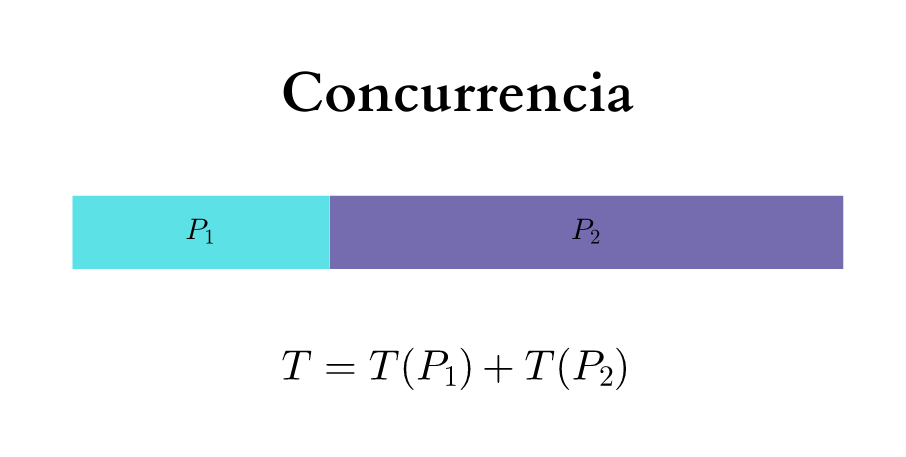
\includegraphics[width=5cm]{concurrencia.png}
\end{center}

En la computación paralela, la ejecución ocurre en el mismo instante físico, los c\'alculos se realizan de forma verdaderamente simul\'anea. Para maximizar el uso de múltiples procesadores o n\'ucleos, presentes en las CPU modernas, el procesamiento en paralelo dividirá el trabajo entre varios subprocesos, cada uno de los cuales puede ejecutarse de forma independiente en un núcleo diferente.

Sea T el tiempo total de ejecuci\'on de dos programas paralelos $ P_{1} $ y $ P_{2} $:

\begin{center}
	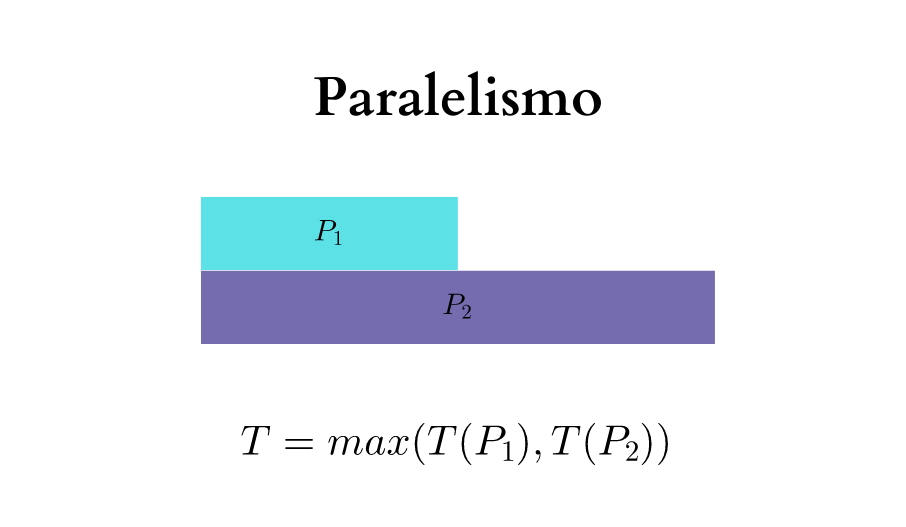
\includegraphics[width=5cm]{paralelismo.png}
\end{center}

Paralelismo implica concurrencia, pero no se cumple el rec\'iproco.

\subsection{Monitors en C\#}
Proporcionan un mecanismo que sincroniza el acceso a los objetos.

La clase Monitor permite sincronizar el acceso a una región de código tomando y liberando un bloqueo en un objeto determinado llamando a los métodos Monitor.Enter, Monitor.TryEnter y Monitor.Exit . Los bloqueos de objeto proporcionan la capacidad de restringir el acceso a un bloque de código, normalmente denominado sección crítica. Aunque un subproceso posee el bloqueo de un objeto, ningún otro subproceso puede adquirir ese bloqueo. También puede usar la Monitor clase para asegurarse de que ningún otro subproceso pueda acceder a una sección del código de aplicación que ejecuta el propietario del bloqueo, a menos que el otro subproceso ejecute el código mediante un objeto bloqueado diferente.

\subsection{Sem\'aforos en C\#}

\subsection{Barriers en C\#}

Permite que múltiples tareas trabajen de manera cooperativa en un algoritmo en paralelo a través de múltiples fases.

En esta sincronización de barrera, tenemos varios subprocesos que trabajan en un solo algoritmo. El algoritmo funciona en fases. Todos los subprocesos deben completar la fase 1 y luego pueden continuar con la fase 2. Hasta que todos los subprocesos no completen la fase 1, todos los subprocesos deben esperar a que todos los subprocesos lleguen a la fase 1.

\subsection{Countdowns en C\#}

\subsection{Propuesta en Go para la sincronización en la concurrencia}

\subsection{Solución a los filósofos}

\subsubsection{Go}

\subsubsection{C\#}

\subsubsection{Comparaci\'on}
%----------------------------------------------------------------------------------------

\end{document}
